\documentclass[tikz, border=8pt]{standalone}
\usepackage[T1]{fontenc}
\usepackage{tgpagella}
\usepackage{mathpazo}
\usepackage{tikz}
\usepackage{amsmath}
\usepackage{amssymb}
\usepackage{xcolor}
\usepackage{fontawesome5}
\usetikzlibrary{positioning, arrows.meta, shapes.geometric, fit, backgrounds, calc}

% ----------------------------------------------------------------
% Inline palette -- mirrors figures/_palette.tex (AGENTS.md rule 1).
% Kept inline so this figure compiles stand-alone regardless of
% TEXINPUTS, matching figures/architecture.tex.
% ----------------------------------------------------------------
\definecolor{cAudio}{HTML}{F5EFE3}
\definecolor{cEnc}{HTML}{DDE9EC}
\definecolor{cEncB}{HTML}{2D8294}
\definecolor{cAdp}{HTML}{F0DFC9}
\definecolor{cAdpB}{HTML}{B07849}
\definecolor{cLLM}{HTML}{F4E6D5}
\definecolor{cLLMB}{HTML}{A0763C}
\definecolor{cPrompt}{HTML}{F1ECE3}
\definecolor{cPromptB}{HTML}{8E7A55}
\definecolor{cTok}{HTML}{E5EEF0}
\definecolor{cTokB}{HTML}{5E8090}
\definecolor{cBound}{HTML}{ECDFD3}
\definecolor{cBoundB}{HTML}{9C7558}

\newcommand{\frozenIcon}{\textcolor{cEncB}{\faSnowflake}}
\newcommand{\fireIcon}{\textcolor{cLLMB!90!red}{\faFire}}

\newcommand{\WaveformPictogram}{%
  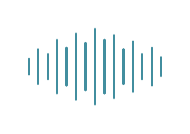
\begin{tikzpicture}[baseline=-0.6ex]
    \foreach \i/\h in {%
        0/0.10, 1/0.22, 2/0.16, 3/0.34, 4/0.24,
        5/0.42, 6/0.30, 7/0.48, 8/0.34, 9/0.40,
        10/0.22, 11/0.32, 12/0.16, 13/0.24, 14/0.12%
    }{
      \pgfmathsetmacro{\xpos}{-0.84 + \i*0.12}
      \draw[line width=0.85pt, line cap=round, draw=cEncB!90]
        (\xpos, -\h) -- (\xpos, \h);
    }
  \end{tikzpicture}%
}

\tikzset{
  module/.style    ={draw, rounded corners=3pt, align=center,
                     font=\small, line width=0.7pt,
                     minimum width=5.0cm, minimum height=1.0cm},
  audio/.style     ={module, fill=cAudio, draw=black!35,
                     minimum width=2.8cm, minimum height=1.0cm},
  llmbox/.style    ={module, fill=cLLM, draw=cLLMB, line width=0.85pt,
                     minimum height=1.0cm, font=\normalsize},
  retrieverbox/.style = {module, fill=cBound, draw=cBoundB,
                         minimum height=1.1cm},
  gapcheck/.style    = {module, fill=cBound!60, draw=cBoundB, dashed,
                        minimum height=1.1cm},
  hpool/.style       = {draw=cAdpB, fill=cAdp, line width=0.75pt,
                        cylinder, shape border rotate=90,
                        aspect=0.22,
                        minimum width=2.6cm, minimum height=2.2cm,
                        align=center, font=\small},
  dashedmod/.style   = {module, fill=cTok!50, draw=cTokB, dashed,
                        line width=0.6pt, minimum width=3.2cm,
                        minimum height=0.95cm, font=\small},
  outbox/.style      = {module, fill=white, draw=black!50,
                        minimum width=3.6cm, minimum height=0.85cm},
  flow/.style        = {-Stealth, line width=0.7pt, draw=black!70},
  dashedflow/.style  = {flow, dashed, draw=black!55},
  edgelabel/.style   = {font=\scriptsize, text=black!55, fill=white, inner sep=1pt},
  paneltitle/.style  = {font=\bfseries\small, align=center, text=cLLMB},
  paneltitleaud/.style = {font=\bfseries\small, align=center, text=cTokB},
  promptsnip/.style  = {font=\scriptsize, align=left,
                        draw=cAdpB!60, dashed, rounded corners=2pt,
                        fill=cAdp!30, inner sep=3pt},
}

\begin{document}
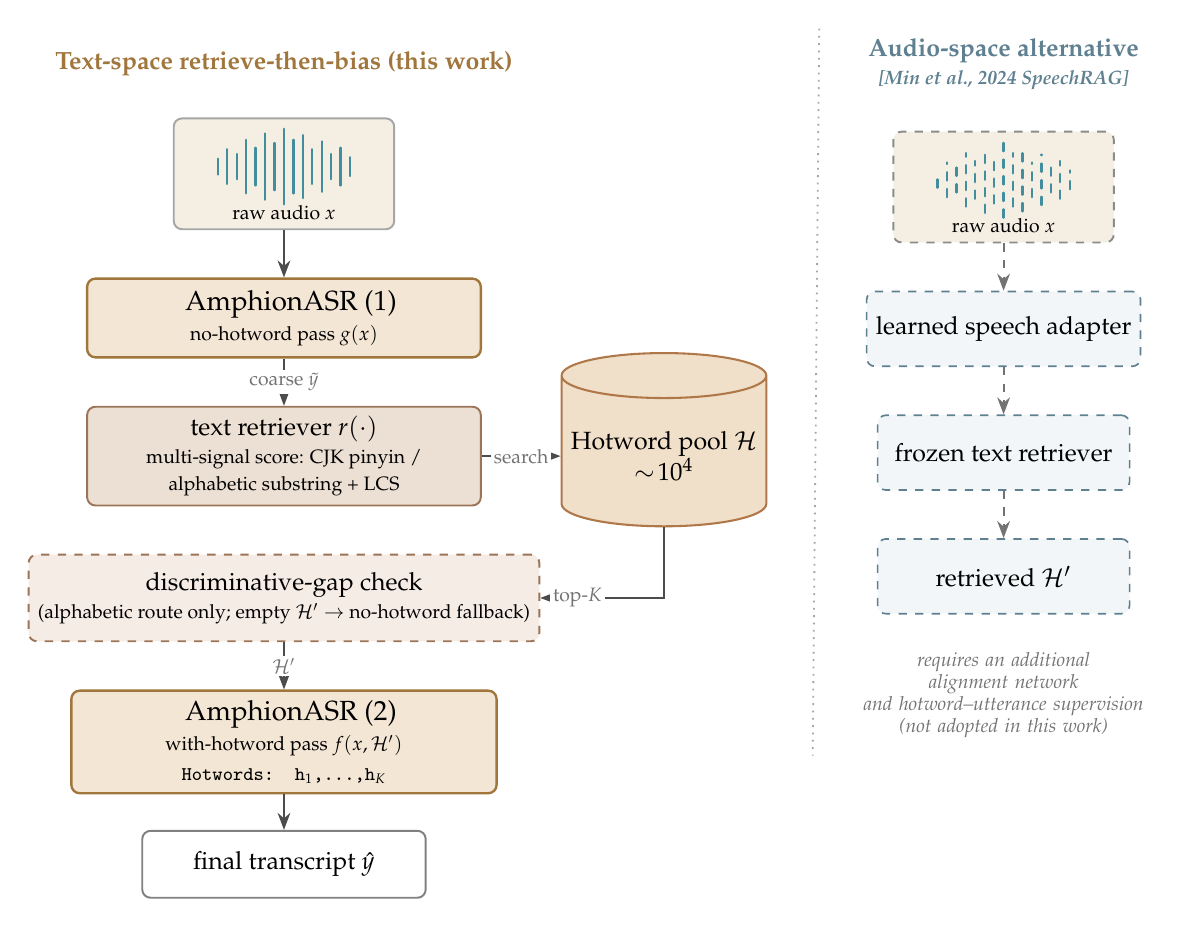
\begin{tikzpicture}[node distance=0.6cm and 0.65cm]

  % ============================================================
  % LEFT PANEL -- Text-space retrieve-then-bias (this work)
  % ============================================================
  \node[paneltitle] (lt) {Text-space retrieve-then-bias (this work)};

  \node[audio, below=0.4cm of lt] (wave)
    {\WaveformPictogram\\[-1pt]{\scriptsize raw audio $x$}};

  \node[llmbox, below=of wave] (g)
    {\fireIcon~~AmphionASR (1)\\[-1pt]
     {\scriptsize no-hotword pass $g(x)$}};

  \node[retrieverbox, below=of g] (retr)
    {text retriever $r(\cdot)$\\[-1pt]
     {\scriptsize multi-signal score: CJK pinyin /}\\[-1pt]
     {\scriptsize alphabetic substring + LCS}};

  \node[gapcheck, below=of retr] (gap)
    {discriminative-gap check\\[-1pt]
     {\scriptsize (alphabetic route only; empty $\mathcal{H}'$ $\to$ no-hotword fallback)}};

  \node[llmbox, below=of gap, minimum width=5.4cm] (f)
    {\fireIcon~~AmphionASR (2)\\[-1pt]
     {\scriptsize with-hotword pass $f(x, \mathcal{H}')$}\\[-1pt]
     {\scriptsize\ttfamily Hotwords: h$_1$,\ldots,h$_K$}};

  \node[outbox, below=0.45cm of f] (yhat)
    {final transcript $\hat{y}$};

  \node[hpool, right=1.0cm of retr.east, anchor=west] (pool)
    {Hotword pool $\mathcal{H}$\\$\sim\!10^4$};

  % --- Arrows in left panel ---
  \draw[flow] (wave) -- (g);
  \draw[flow] (g) -- (retr) node[midway, edgelabel] {coarse $\tilde{y}$};
  \draw[flow] (retr.east) -- (pool.west) node[midway, edgelabel] {search};
  \draw[flow] (pool.south) |- (gap.east) node[pos=0.85, edgelabel] {top-$K$};
  \draw[flow] (gap) -- (f) node[midway, edgelabel] {$\mathcal{H}'$};
  \draw[flow] (f) -- (yhat);

  % ============================================================
  % RIGHT PANEL -- Audio-space alternative (dashed contrast only)
  % ============================================================
  \coordinate (rcenter) at ($(pool.east) + (3.0, 0)$);

  \node[paneltitleaud] (rt) at (rcenter |- lt)
    {Audio-space alternative\\[-1pt]
     {\scriptsize\itshape [Min et al., 2024 SpeechRAG]}};

  \node[audio, dashed, draw=black!45, below=0.4cm of rt] (rwave)
    {\WaveformPictogram\\[-1pt]{\scriptsize raw audio $x$}};
  \node[dashedmod, below=of rwave]     (radapter) {learned speech adapter};
  \node[dashedmod, below=of radapter]  (rretr)    {frozen text retriever};
  \node[dashedmod, below=of rretr]     (rH)       {retrieved $\mathcal{H}'$};

  \draw[dashedflow] (rwave)    -- (radapter);
  \draw[dashedflow] (radapter) -- (rretr);
  \draw[dashedflow] (rretr)    -- (rH);

  \node[font=\scriptsize\itshape, text=black!55, align=center,
        below=0.35cm of rH, text width=3.6cm] (rnote)
    {requires an additional alignment network\\and
     hotword--utterance supervision\\(not adopted in this work)};

  % --- Visual divider between panels ---
  \draw[dotted, line width=0.65pt, draw=black!35]
       ($(rt.west) + (-0.5, 0.45)$) -- ($(rnote.south west) + (-0.5, -0.1)$);

\end{tikzpicture}
\end{document}
